\documentclass[titlepage, a4paper, openbib, 10pt]{article}

%#####################################
%Usepackages en installingen
\usepackage[top=1in, bottom=1in, left=1in, right=1in]{geometry}
\usepackage[pdftex]{graphicx}
\usepackage{fancyhdr}
\usepackage{sectionbox}
\usepackage[dutch]{babel}
\usepackage{chngcntr}
\usepackage{cite}
\usepackage{url}
\usepackage{makeidx}
\usepackage{paralist}
\usepackage{enumitem}
\usepackage{tocloft}
\usepackage{listliketab}	
\usepackage[table]{xcolor}
\usepackage{tabularx}
\usepackage{epsfig}
\usepackage{pdflscape}
\usepackage{pdfpages}
\usepackage{float}
\usepackage{multirow} 
\usepackage{rotating}
\usepackage[utf8]{inputenc}
\usepackage{color}
\usepackage{fp}
\newcommand{\red}[1]{
\textcolor{red}{#1}
}
\usepackage{listings}
\lstset{language=C,
basicstyle=\ttfamily\footnotesize,
frame=shadowbox,
mathescape=true,
showstringspaces=false,
showspaces=false,
breaklines=true}


%\usepackage{showframe} %tmp
%#####################################
%Nieuwe commando's
\newcommand{\HRule}{\rule{\linewidth}{1pt}}
\newcommand{\organisatie}{\uppercase{Hogeschool Rotterdam / CMI}}
\newcommand{\modulenaam}{Development 1}
\newcommand{\modulecode}{\uppercase{INFDEV02-1}}
\newcommand{\studiejaar}{\uppercase{2016-2017}}
\newcommand{\stdPunten}{4}
\renewcommand{\author}{Dr. Giuseppe Maggiore, Tony Busker}

\definecolor{lichtGrijs}{RGB}{169,169,169}



%#####################################
%Index en styling
\setlength{\cftbeforesecskip}{10pt}
\setlength\parindent{0pt}
\makeindex
\graphicspath{{../img/}}
\counterwithin{figure}{subsection}
\pagestyle{fancy}
\setcounter{secnumdepth}{5}
\setcounter{tocdepth}{5}

%#####################################
%     Alles voor header/footer
\fancyhf[HL]{\nouppercase{\textit{\leftmark}}}
\setlength{\headheight}{36pt}
\lhead{\uppercase{\footnotesize Course description}}
\chead{\footnotesize \organisatie}
\rhead{
\includegraphics[width=0.09\textwidth]{logo}}

\lfoot{\scriptsize \modulenaam}
\cfoot{\scriptsize \today}
\rfoot{\small \thepage}

\renewcommand{\headrulewidth}{0.4pt}
\renewcommand{\footrulewidth}{0.4pt}
%#####################################

\begin{document}

%#####################################
%Titlepage
\begin{titlepage}
\thispagestyle{fancy}
\ 
\vspace{5cm}

\begin{center}

	
	\Large \textbf \organisatie
	
	\vspace{1.5cm}
	
	\HRule \\[0.4cm]
	
	\Huge \textbf \modulenaam
	
	\vspace{1.7cm}
	
	\Large \textbf  \modulecode
	
	\vspace{0.4cm}
	
	\HRule \\[1.5cm]
\end{center}
\vfill

% Author and supervisor
\begin{tabular}{l l}
	Number of study points:  & \stdPunten{} ects\\
	Course owners: & \author\\
\end{tabular}

\end{titlepage}

%####### Contentpagina ########
%\renewcommand{\baselinestretch}{1.5}\normalsize
%\tableofcontents
%\newpage
%\listoffigures
%\newpage
%\listoftables
%\newpage

%########### Inhoud ###########

\shadowsectionbox
\section*{Modulebeschrijving}
\begin{tabularx}{\textwidth}{|>{\columncolor{lichtGrijs}} p{.26\textwidth}|X|}
	\hline
	\textbf{Module name:} & \modulenaam\\
	\hline
	\textbf{Module code: }& \modulecode\\
	\hline
	\textbf{Study points \newline and hours of effort:} & This module gives \stdPunten{}  ects, in correspondence with \FPeval{\result}{clip(\stdPunten*28)}\result{} hours:
	\begin{itemize}
		\item 3 x 6 hours frontal lecture
		\item 3 x 6 hours practicum
		\item the rest is self-study
	\end{itemize} \\
	\hline
	\textbf{Examination:} & Written examination and practicums (with oral check) \\
	\hline
	\textbf{Course structure:} & Lectures, self-study, and practicums \\
	\hline
	\textbf{Prerequisite knowledge:} & None. \\
	\hline
	\textbf{Learning tools:}  &
		\begin{itemize}
			\item Book: Think Python; author A. B. Downey (\url{http://www.greenteapress.com/thinkpython/})
			\item Presentations (in pdf): found on N@tschool and on the GitHub repository \url{https://github.com/hogeschool/INFDEV02-1}
			\item Assignments, to be done at home and during practical lectures (pdf): found on N@tschool and on the GitHub repository \url{https://github.com/hogeschool/INFDEV02-1}
		\end{itemize} \\
	\hline
	\textbf{Connected to \newline competences:} &
	\begin{center}
		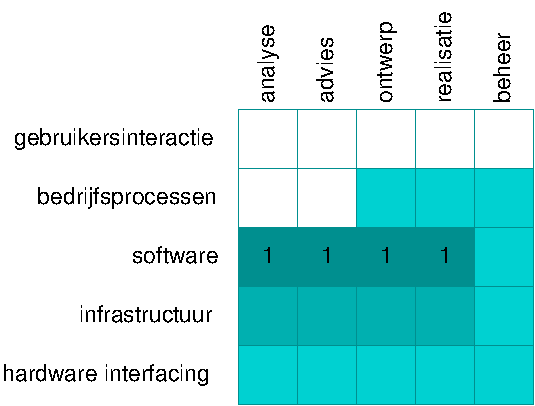
\includegraphics[width=7cm]{../img/comptabel.pdf}
	\end{center}\\
	\hline
	\textbf{Learning objectives:} &
		At the end of the course, the student can:
			\begin{itemize}
				\item \textbf{understand} and \textbf{describe} the logical model of computation \texttt{LMC}
				\item \textbf{understand} and \textbf{describe} the concrete model of computation \texttt{CMC}
				\item \textbf{use} variables and basic data types \texttt{VAR}
				\item \textbf{use} arithmetic and boolean expressions \texttt{EXPR}
				\item \textbf{use} conditional control-flow statements \texttt{COND}
				\item \textbf{use} looping control-flow statements \texttt{LOOP}
			        \item \textbf{understand} the concept of abstraction through function definition \texttt{FUNABS}
                                \item \textbf{use} and \textbf{design} functions \texttt{FUNDEF}
			\end{itemize} \\
		
	\hline
\end{tabularx}
\newpage

\begin{tabularx}{\textwidth}{|>{\columncolor{lichtGrijs}} p{.26\textwidth}|X|}
	\hline
	\textbf{Content:}&
	\begin{itemize}
		\item basic concepts of computation from a logical standpoint
		\item basic concepts of computation from a concreter perspective in terms of storage and instructions
		\item variables (in Python 3)
		\item primitive datatypes and expressions (in Python 3)
		\item conditional control-flow statements (in Python 3)
		\item looping control-flow statements (in Python 3)
	\end{itemize} \\
	\hline
	\textbf{Course owners:} & \author\\
	\hline
	\textbf{Date:} & \today \\
	\hline
\end{tabularx}
\newpage

\newpage
\section{General description}
		Programming is one of the most ubiquitous activities within the field of ICT. Many business needs are centered around the gathering, elaboration, simulation, etc. of data through programs. \\
		
		This course covers the very basic aspects of programming in the Python programming language (version 3). \\

	\subsection{Relationship with other teaching units}
		All subsequent programming courses build upon the knowledge learned during this course.	\\
		
		Knowledge acquired through the programming courses is also useful for the projects. A word of warning though: projects and development courses are largely independent, so some things that a student learns during the development courses are not used in the projects, some things that a student learns during the development courses are indeed used in the projects, but some things done in the projects are learned within the context of the project and not within the development courses.

\newpage
\section{Course program}
	The course is structured into six lectures. The six lectures take place during the six weeks of the course, but are not necessarily in a one-to-one correspondance with the course weeks. For example, lectures one and two are fairly short and will take place during a single week.

	\subsection{Lecture 1 - logical model of computation}
		The first lecture covers basic concepts of computation from a logical standpoint.

		\paragraph*{Topics}
			\begin{itemize}
				\item Following a path (example: \textit{take three steps forward, turn left, ...});
				\item Following a path with state (example: \textit{read N from the whiteboard, take N steps forward, ...});
				\item Following a path with wrongly typed state (example: \textit{take Monday steps forward, ...});
				\item Following a path with state and conditionals (example: \textit{take N steps forward if the lecturer is smiling, ....}).
			\end{itemize}

		\paragraph*{Activities}
			\begin{itemize}
				\item Let students follow instructions;
				\item Introduce elements of state and let students follow instructions with state (\textit{take N/4 steps forward; N is your age});
				\item Introduce elements of writable state and let students follow instructions with writable state (\textit{take N/4 steps forward; N is written under the yellow sticker});
				\item Introduce elements of decision-making and let students follow instructions with state and decision making (\textit{if the sun is shining, then take N/4 steps forward; otherwise, go sit down});
				\item Introduce elements of iteration and let students follow instructions with state, decision making, and iteration (\textit{divide the students in teams, and let run some script battling for the toy farm}).
			\end{itemize}

			\subsection{Lecture 2 - concrete model of computation}
				The second lecture covers basic concepts of computation from a concreter perspective in terms of storage and instructions.

				\paragraph*{Topics}
					\begin{itemize}
						\item CPU and memory;
						\item a basic overview of the various things that an imperative language can do, independent of syntax;
						\item introduction to semantics and post-conditions.
					\end{itemize}

				\paragraph*{Activities}
					\begin{itemize}
						\item Formalize the concept of instructions seen in the previous lecture by rewriting the scripts;
						\item Formalize the concept of state and mutation seen in the previous lecture by rewriting the scripts;
						\item Formalize the concept of decision-making seen in the previous lecture by rewriting the scripts;
						\item Formalize the concept of iteration seen in the previous lecture by rewriting the scripts.
					\end{itemize}


			\subsection{Lecture 3 - Hello Python! and variables}
				The third lecture covers an introduction to Python and its concept of variables.

				\paragraph*{Topics}
					\begin{itemize}
						\item brief history of programming languages;
						\item brief introduction to Python: what it does, what it does not, why we have chosen it;
						\item variables in python for integers;
						\item the effect of variable assignment on memory;
					\end{itemize}

			\subsection{Lecture 4 - datatypes, and expressions}
				The fourth lecture covers primitive datatypes and their associated expressions in the Python programming language.

				\paragraph*{Topics}
					\begin{itemize}
						\item what are data-types and \textit{why we do need them}?
						\item different Python data-types;
						\item arithmetic expressions;
						\item integer and floating point operators;
						\item boolean expressions;
						\item conditional expressions;
						\item very long expressions with conditionals vs temporary variables: the art of naming to encode knowledge.
					\end{itemize}

				\paragraph*{Activities}
					Call upon students to solve small riddles related to sample Python scripts on:

					\begin{itemize}
						\item Integers, strings, floats, bools;
						\item Integer, string, float, and bool varialbes;
						\item Semantics and post-conditions on variable-assignments.
						\item Integers, strings, floats, bool expressions;
						\item Conditional expressions;
						\item Semantics and post-conditions on expressions and conditional expressions.
					\end{itemize}

			\subsection{Lecture 5 - conditional control-flow statements}
				The fifth lecture covers conditional control-flow statements in the Python programming language.

				\paragraph*{Topics}
					\begin{itemize}
						\item making choices;
						\item \texttt{if-then} statements;
						\item \texttt{if-then-else} statements;
						\item the importance of an \texttt{else} statement;
						\item (slightly informal) semantics;
						\item exponential explosion of potential control-paths;
						\item expressive power of \texttt{if-then-else}.
					\end{itemize}

				\paragraph*{Activities}
					Call upon students to solve small riddles related to sample Python scripts on:

					\begin{itemize}
						\item \texttt{if-then} and \texttt{if-then-else} statements;
						\item how many possible final states of a program;
						\item semantics and post-conditions on conditional statements.
					\end{itemize}


			\subsection{Lecture 6 - looping control-flow statements}
				The sixth (and last) lecture covers looping control-flow statements in the Python programming language.

				\paragraph*{Topics}
					\begin{itemize}
						\item repeated behaviors;
						\item \texttt{while} statements;
						\item (slightly informal) semantics;
						\item (more than) exponential explosion of potential control-paths;
						\item expressive power of \texttt{while};
						\item \texttt{for} statements;
						\item (slightly informal) semantics;
						\item \texttt{for} as a \textit{limited} form of \texttt{while}.
					\end{itemize}

				\paragraph*{Activities}
					Call upon students to solve small riddles related to sample Python scripts on:

					\begin{itemize}
						\item \texttt{while} and \texttt{for} loops;
						\item how many possible final states of a program;
						\item semantics and post-conditions on loops.
					\end{itemize}

\newpage
\section{Assessment}
The course is tested with two exams: a series of practical assignments, a brief oral check of sthe practical assignments, and a theoretical exam. The final grade is determined as follows: \\

\texttt{if theoryGrade $\geq$ 75\% \& practicumCheckOK then return practicumGrade else return insufficient}

This means that the theoretical knowledge is a strict requirement in order to get the actual grade from the practicums, but it does not reflect your level of skill and as such does not further influence your grade.

\paragraph*{Motivation for grade}
A professional software developer is required to be able to program code which is, at the very least, \textit{correct}.

In order to produce correct code, we expect students to show:
\begin{inparaenum}[\itshape i\upshape)]
\item a foundation of knowledge about how a programming language actually works in connection with a simplified concrete model of a computer;
\item fluency when actually writing the code.
\end{inparaenum}

The quality of the programmer is ultimately determined by his actual code-writing skills, therefore the final grade comes only from the practicums. The quick oral check ensures that each student is able to show that his work is his own and that he has adequate understanding of its mechanisms. The theoretical exam tests that the required foundation of knowledge is also present to avoid away of programming that is exclusively based on intuition, but which is also grounded in concrete and precise knowledge about what each instruction does.


\subsection{Theoretical examination DEV I}
The general shape of a theoretical exam for \texttt{DEV I} is made up of a series of highly structured open questions. In each exam the content of the questions will change, but the structure of the questions will remain the same. For the structure (and an example) of the theoretical exam, see the appendix.


\subsection{Practical examination DEV I}
...


\newpage
\section*{Exam structure}
What follows is the general structure of a \modulecode exam.

\paragraph{Question I: formal rules} \ \\

\textbf{General shape of the question:} \textit{given a set of rules, and given the starting point, what is the result of excution? Give the intermediate steps as well.}

\ \\ 

\textbf{Points:} \textit{25\%.}

\ \\ 

\textbf{Grading:} \textit{All points for correct answer, partial trajectories count for exactly half the score, a completely orthogonal trajectory counts for no points.}

\ \\ 

\textbf{Associated learning goals:} \texttt{LMC}.

\ \\ 

\paragraph{Question II: program state} \ \\ 

\textbf{General shape of the question:} \textit{Fill-in the program state with the values that the variables assume while running the sample below.}

\ \\ 

\textbf{Points:} \textit{25\%.}

\ \\ 

\textbf{Grading:} \textit{Full points if all stack frames and return types are correctly listed, with the right time stamps. Half points if at least half of all stack frames is listed. Zero points otherwise.}

\ \\ 

\textbf{Associated learning goals:} \texttt{CMC}.

\ \\ 

\paragraph{Question III: variables, expressions, and data types}

\ \\ 

\textbf{General shape of the question:} \textit{What is the value and the type of all variables after execution of the following code?}

\ \\ 

\textbf{Points:} \textit{25\%.}

\ \\ 

\textbf{Grading:} \textit{All values and types are correct: full-points. At least half the values and at least half the types are correct: half points. Zero points otherwise.}

\ \\ 

\textbf{Associated learning goals:} \texttt{VAR}, \texttt{EXPR}.

\ \\ 

\paragraph{Question IV: control flow}

\ \\ 

\textbf{General shape of the question:} \textit{What is the value of all variables after execution of the following code?}

\ \\ 

\textbf{Points:} \textit{25\%.}

\ \\ 

\textbf{Grading:} \textit{All values are correct: full-points. At least half the values are correct: half points. Zero points otherwise.}

\ \\ 

\textbf{Associated learning goals:} \texttt{COND}, \texttt{LOOP}.

\ \\ 

\newpage
\section*{Exam sample}
What follows is a concrete example of the exam.


\paragraph{Question I: formal rules} \ \\

\textit{You start at point (0,0). Take a step in the direction (10,0) until you are above point (45,0). Then take five steps in the direction (0,2). Where do you end up?}

\ \\ 

\textbf{Answer:} \textit{The trajectory is:}

\begin{lstlisting}

P1 = (50,0)
 +----- P2 = (50,10)
 |
 |
 |
 |
P0 = (0,0)
\end{lstlisting}

\ \\ 

\textbf{Points:} \textit{25\%.}

\ \\ 
\ \\ 

\paragraph{Question II: program state} \ \\ 

\textit{Fill-in the program state with the values that the variables assume while running the sample below.}

\begin{lstlisting}
y = 1
for i in range(0, 5):
    y = y * 2
\end{lstlisting}

\ \\ 

\textbf{Answer:} \textit{The variable allocations are:}

\begin{tabular}{| c | c | c | c | c | c | c | c | c | c | c | c |}
\hline
\textbf{y} & 1    & 1 & 2 & 2 & 4 & 4 & 8 & 8 & 16 & 16 & 32 \\
\hline
\textbf{i} & n.a. & 0 & 0 & 1 & 1 & 2 & 2 & 3 & 3  &  4 &  4 \\
\hline
\end{tabular}

\ \\

\textbf{Points:} \textit{25\%.}

\ \\ 

\textbf{Grading:} \textit{Full points if all values are correctly listed in the right order. Half points if at least half of values are listed in the right order. Zero points otherwise.}

\ \\ 

\textbf{Associated learning goals:} \texttt{CMC}.

\ \\ 

\paragraph{Question III: variables, expressions, and data types}

\ \\ 

\textit{What is the value and the type of all variables after execution of the following code?}
\begin{lstlisting}
v = 0
i = "Hello + world"
j = "Hello" + "world"
k = 10 / 3
l = 10 / 3.0
\end{lstlisting}

\ \\ 

\textbf{Answer:} \textit{The value and type of all variables after execution is:}

\begin{tabular}{| l | c | c | }
\hline
\textbf{Variable} & \textbf{Value} & \textbf{Type} \\
\hline
v & 0 & int \\
\hline
i & 'Hello + world' & str \\
\hline
j & 'Helloworld' & str \\
\hline
k & 3 & int \\
\hline
l & 3.3333$\dots$ & float \\
\hline
\end{tabular}

\ \\ 

\textbf{Points:} \textit{25\%.}

\ \\ 

\textbf{Grading:} \textit{All values and types are correct: full-points. At least half the values and at least half the types are correct: half points. Zero points otherwise.}

\ \\ 

\textbf{Associated learning goals:} \texttt{VAR}, \texttt{EXPR}.

\ \\ 

\paragraph{Question IV: control flow}

\ \\ 

\textbf{General shape of the question:} \textit{What is the value of all variables after execution of the following code?}

\ \\ 

\textbf{Concrete example of question:} \textit{What is the value of all variables after execution of the following code?}

\begin{lstlisting}
v = 0
for i in range(1,15):
  if (i % 2 == 0) & (i % 3 == 0):
    v = v + i
\end{lstlisting}

\ \\ 

\textbf{Concrete example of answer:} \textit{The value of all variables after execution is:}

\begin{tabular}{| l | c |}
\hline
\textbf{Variable} & \textbf{Value} \\
\hline
\texttt{i} & \texttt{14} \\
\hline
\texttt{v} & \texttt{18} \\
\hline
\end{tabular}

\ \\ 

\textbf{Points:} \textit{25\%.}

\ \\ 

\textbf{Grading:} \textit{All values are correct: full-points. At least half the values are correct: half points. Zero points otherwise.}

\ \\ 

\textbf{Associated learning goals:} \texttt{COND}, \texttt{LOOP}.

\ \\ 

%##############################

\newpage
%\bibliographystyle{plain}
%\bibliography{references}
%\newpage
\section*{Bijlage 1: Toetsmatrijs}
	\begin{tabular}{|p{1cm}|p{4cm}|}
		\hline
		Learning goals & Dublin descriptors \\
		\hline
		\texttt{LMC} & 1, 4 \\
		\hline
		\texttt{CMC} & 1, 4 \\
		\hline
		\texttt{VAR} & 1, 2, 4 \\
		\hline
		\texttt{EXPR} & 1, 2, 4 \\
		\hline
		\texttt{COND} & 1, 2, 4 \\
		\hline
		\texttt{LOOP} & 1, 2, 4 \\
		\hline
	\end{tabular}
	
	\vspace{1cm}

	Dublin-descriptors:
	\begin{enumerate}
		\item Knowledge and understanding
		\item Applying knowledge and understanding
		\item Making judgements
		\item Communication
		\item Learning skills
	\end{enumerate}

%\newpage
%\section*{Bijlage 2: Voorbeeldtoets}

		Dit hoofdstuk bevat de beschrijving van de procedures om voor beoordeling in aanmerking te komen.\\
		Bijvoorbeeld voldoende aanwezigheid, 80\% van de opdrachten hebben ingeleverd, presentaties hebben verricht etc.\\

		Verder wordt zo gedetailleerd mogelijk beschreven hoe er tot een cijfer wordt gekomen en welke rollen er door docenten en ander betrokkenen hierbij vervuld worden. \\

		Geef een verantwoording van de toets; wat wordt getoetst, waarom is voor deze vorm gekozen.\\

		Vul een toetsmatrijs in voor de toets (zie bijlage).\\

		Beschrijf ook duidelijk de \textbf{herkansingsmogelijkheden}. \\

		Neem in geval van een schriftelijk tentamen een voorbeeldtoets op als bijlage.\\
		Geef daarbij per deelvraag het aantal te verdienen punten aan. \\

		Bij een schriftelijk rapport. Geef de beoordelingscriteria aan met daarbij de mogelijke score en de onderlinge weging. \\

		Toetsduur: \\

		Hoe en wanneer krijgt de student feedback?\\
%\newpage
%\section*{Bijlage 3: Studielast normering in ects}

		Dit hoofdstuk bevat de beschrijving van de procedures om voor beoordeling in aanmerking te komen.\\
		Bijvoorbeeld voldoende aanwezigheid, 80\% van de opdrachten hebben ingeleverd, presentaties hebben verricht etc.\\

		Verder wordt zo gedetailleerd mogelijk beschreven hoe er tot een cijfer wordt gekomen en welke rollen er door docenten en ander betrokkenen hierbij vervuld worden. \\

		Geef een verantwoording van de toets; wat wordt getoetst, waarom is voor deze vorm gekozen.\\

		Vul een toetsmatrijs in voor de toets (zie bijlage).\\

		Beschrijf ook duidelijk de \textbf{herkansingsmogelijkheden}. \\

		Neem in geval van een schriftelijk tentamen een voorbeeldtoets op als bijlage.\\
		Geef daarbij per deelvraag het aantal te verdienen punten aan. \\

		Bij een schriftelijk rapport. Geef de beoordelingscriteria aan met daarbij de mogelijke score en de onderlinge weging. \\

		Toetsduur: \\

		Hoe en wanneer krijgt de student feedback?\\
\printindex


\end{document}
